\documentclass[12pt]{article}

\usepackage{float}
\usepackage{wrapfig}
\usepackage{geometry}
\usepackage{amsmath}
\usepackage{caption}
\usepackage{amssymb}
\usepackage{fancyhdr}
\usepackage{graphicx}
\usepackage{subcaption}

\pagestyle{fancy}
\setlength{\headheight}{20pt}

\lhead{5615 Assignment 2}
\chead{Alex Keating}
\rhead{\today}
\begin{document}

\subsection*{Approach Overview}
\subsubsection*{Propagation}
	The overall method for the finite-difference propogation was as follows:
	\begin{itemize}
	\item Allocate an array of size $n\times m$ on the GPU's global memory using \texttt{cudaMallocPitch}
	\item Using \texttt{cudaMemcpy2D}, transferred the array containing the initial conditions initialised form the host to device
	\item Set block dimensions to be $\texttt{1}\times\texttt{block\_size}$. Making the $x$-axis of each block any greater than $1$ is redundant as all communciation is done across the $y$-axis.\\
	\textbf{Note:} Experienced strange bug where my global memory/non-optimised  kernel wouldn't execute for some matrix sizes when $\texttt{dimBlock.x} \neq 1$.
	\item Allocate a shared memory array of size \texttt{2*(block\_size+4}). This will be split into two arrays, \texttt{unew} and \texttt{uold}, containing \texttt{block\_size} elements and the four halo values.
	\item Didn't use texture or constant memory as they are both constant. Didn't utilise surface memory as I deemed keeping everything on shared memory as much as possible would be optimum.
	\item Data from global memory transferred to shared memory array at start of kernel.
	\item Single propagation carried out on shared memory arrays.
	\item Update \texttt{unew} vals transferred back to global memory.
	\item Repeated \texttt{p} times at which point global memory array sent back to RAM. 
	\end{itemize}
\subsubsection*{Reduce}
	Overall method for vector reduction as follows:
	\begin{itemize}
	\item Allocate shared array of size \texttt{block\_size}.
	\item Assign values from array in global memory to shared memory.
	\item Apply a binary reduction, leaving one sum for each block.
	\item Write the \texttt{gridDim} sums back to global memory.
	\item Apply previous steps recursively on the remaing values in each row.
	\item Once each row has been reducded to single value, write back array to RAM using \texttt{cudaMemcpy2D}.
	\item Didn't apply atomics as no threads were trying to access the same point in memory so no need to protect the memory address or sequentialise.
	\end{itemize}
	\pagebreak
\subsection*{Results}
\subsubsection*{Propagation calculation times}
\begin{wrapfigure}{l}{0.5\textwidth}
	\centering
	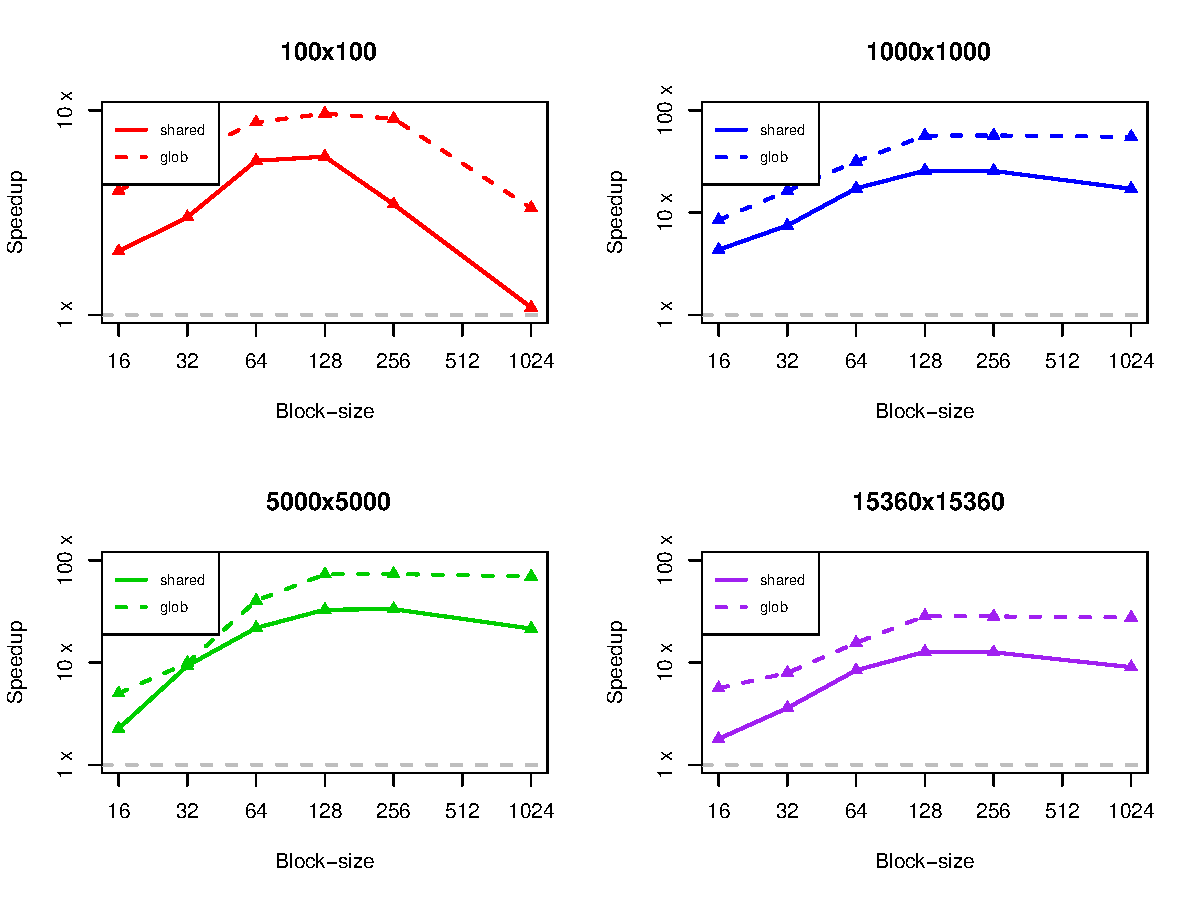
\includegraphics[width=\linewidth]{../plots/fdcalc_sharedvglob.pdf}
	\caption{Speedup of calculation times of finite-difference propogation, comparing global memory and optimisations.}
	\label{fig:3}
\end{wrapfigure}
Figure \ref{fig:1} shows the speedup of the propogation calulation time using the optimised shared memory approach over the CPU's serial time. The speedup reaches up to $\sim33\times$. It increases for the first few increases in matrix size, as expected, however, for $15360\times15360$, there is an evident decrease in speedup. Not clear as to why. Also, interesting to note, there is a clear dip in speedup once the block-size exceeds certain points, depending on the matrix size. For $100\times100$, this is obvious as a block size greater than 128 will be of no benefit to the algorithm.\\
A rather interesting result, is that using the global memory and no optimisations was actually faster than using the shared memory as is seen in Figure \ref{fig:2} and Figure \ref{fig:3}. It can also be seen that for all bar once case, the global memory doesn't experience a slow down as block-size increases, but rather just plateaus. This makes sense as the block-size would have less of an effect when not using shared memory.
\begin{figure}
	\centering
	\begin{subfigure}{0.48\linewidth}
		\centering
		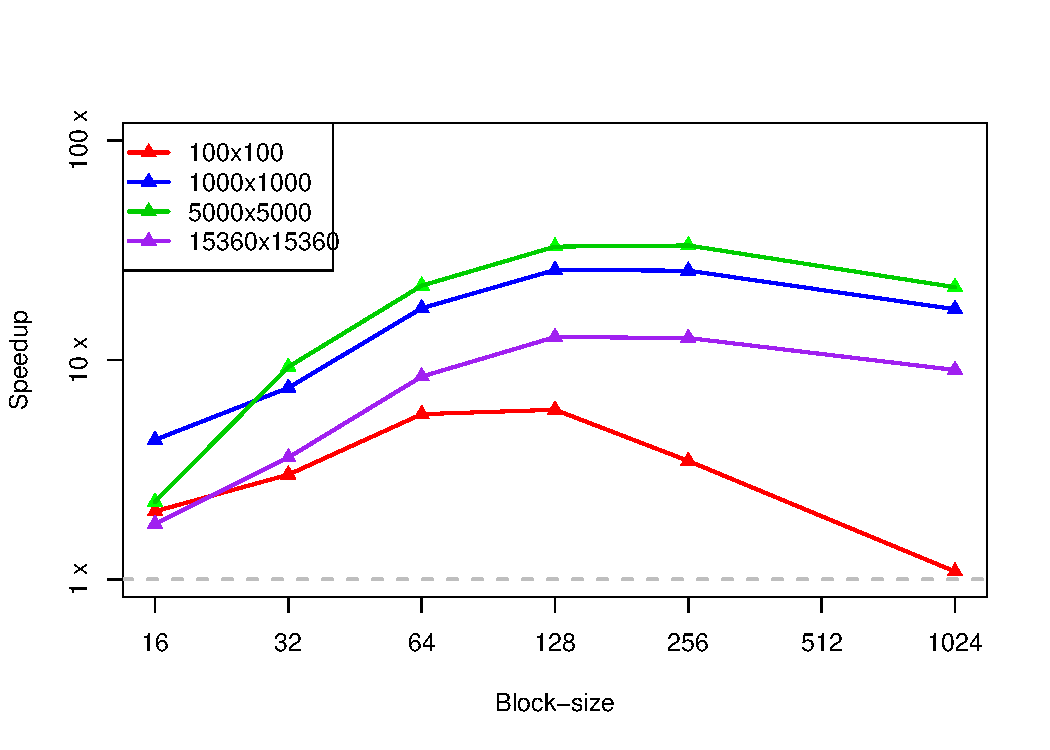
\includegraphics[width=0.85\linewidth]{../plots/fdcalc_shared.pdf}
		\caption{Speedup using shared memory.}
		\label{fig:1}
	\end{subfigure}\hfill
	\begin{subfigure}{0.48\linewidth}
		\centering
		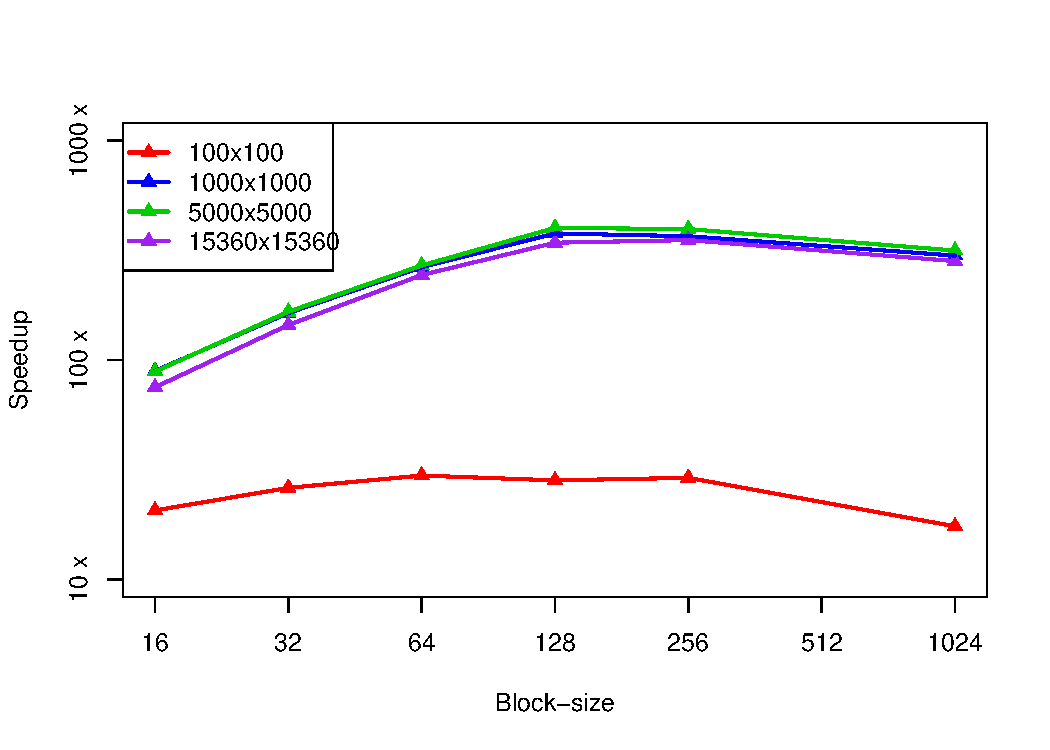
\includegraphics[width=0.85\linewidth]{../plots/fdcalc_glob.pdf}
		\caption{Speedup using global memory.}
		\label{fig:2}
	\end{subfigure}
	\caption{Speedup of calculation times of finite-difference propogation on GPU, using optimisations and using only global memory.}
\end{figure}
\subsubsection*{Reduce calculation times}
\begin{figure}
	\centering
	\begin{subfigure}{0.48\linewidth}
		\centering
		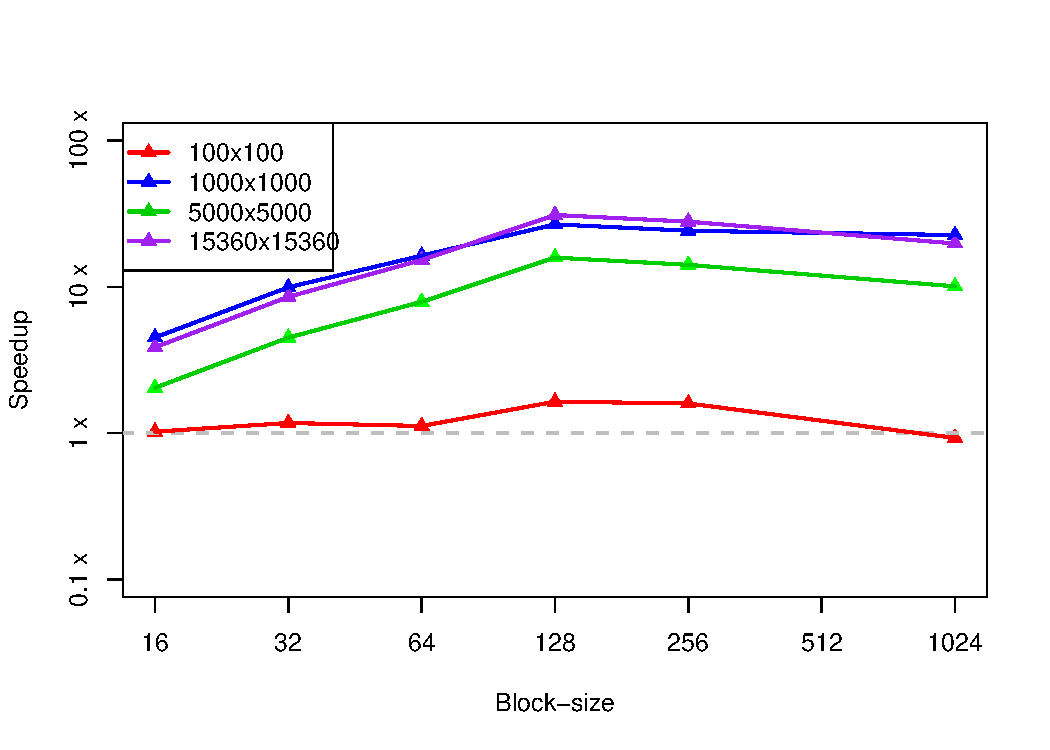
\includegraphics[width=0.85\linewidth]{../plots/redcalc_shared.pdf}
		\caption{Speedup using shared memory.}
		\label{fig:4}
	\end{subfigure}\hfill
	\begin{subfigure}{0.48\linewidth}
		\centering
		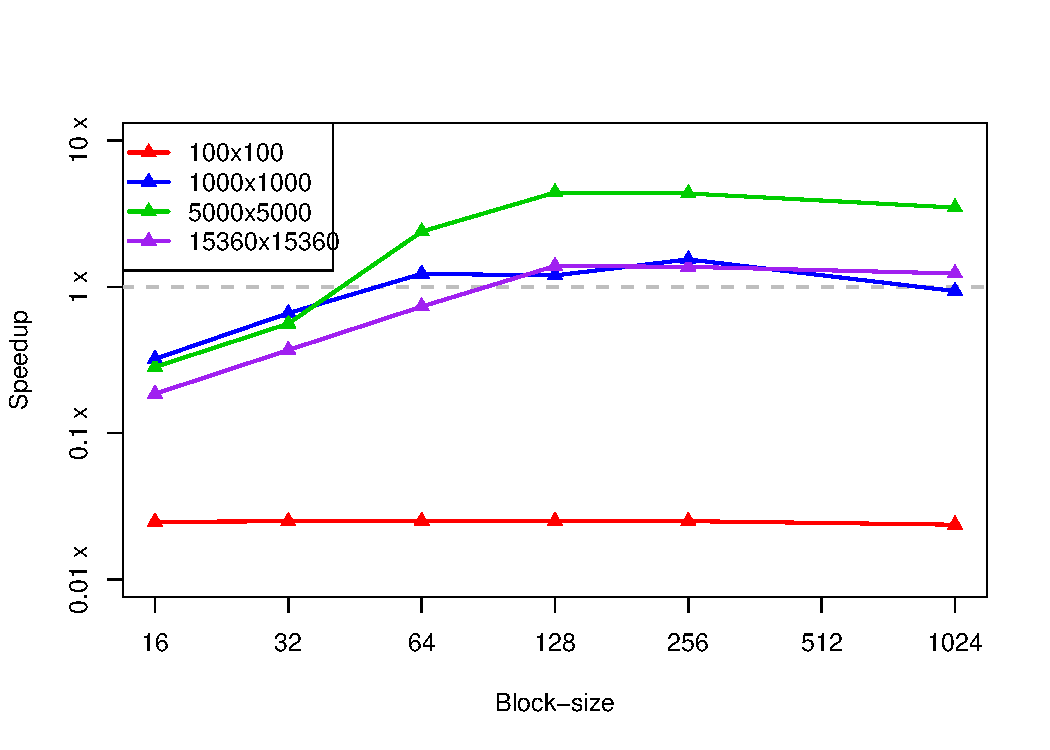
\includegraphics[width=0.85\linewidth]{../plots/redcalc_glob.pdf}
		\caption{Speedup using global memory.}
		\label{fig:5}
	\end{subfigure}
	\caption{Speedup of calculation times of reduce function on GPU, using optimisations and using only global memory.}
\end{figure}
\begin{wrapfigure}{r}{0.5\textwidth}
	\centering
	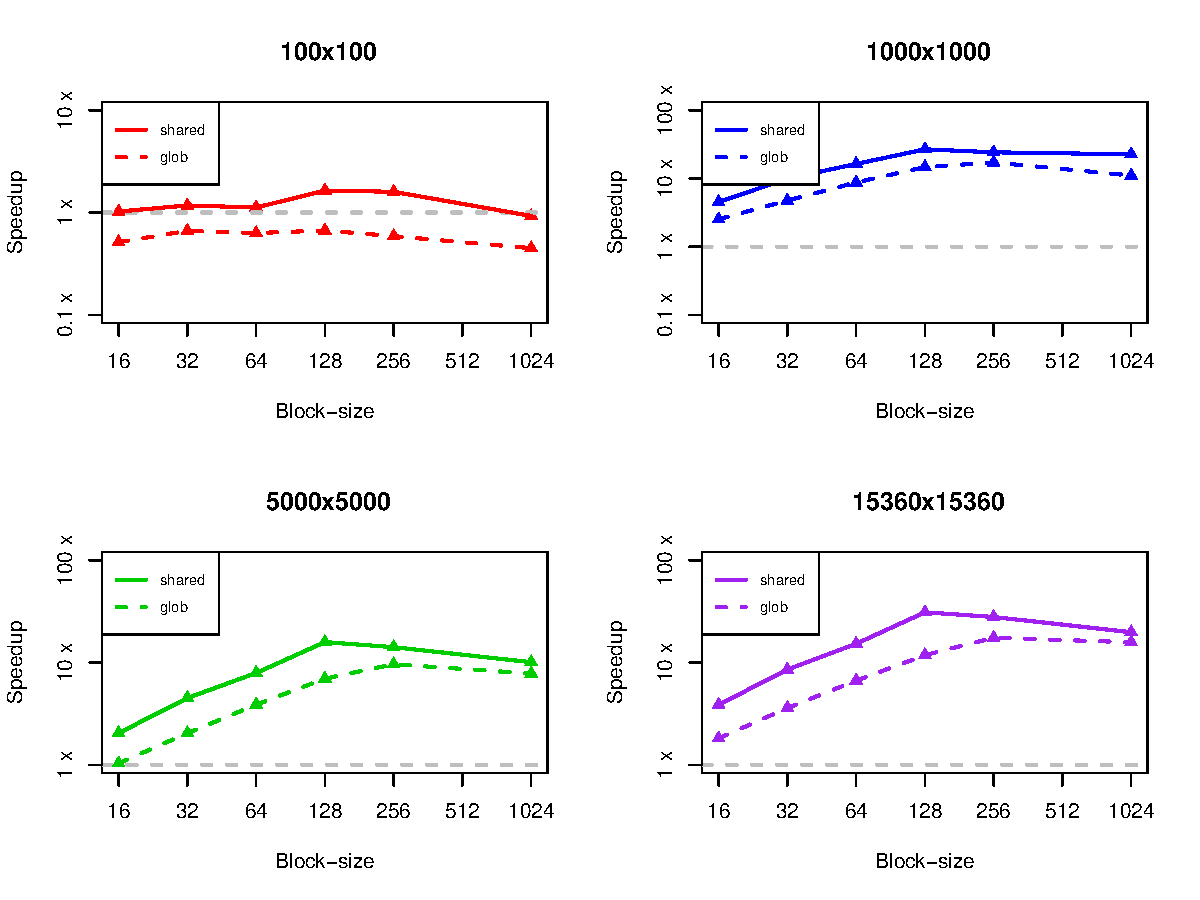
\includegraphics[width=\linewidth]{../plots/red_globvshared.pdf}
	\caption{Speedup of calculation times of reduce function, comparing global memory and optimisations}
	\label{fig:6}
\end{wrapfigure}
The reduce function did not experience the same levels of speedup as seen in the propagation. Presumably due to the increased synchronisation costs of performing the parallelised binary reduction. The results in this case actually started off significantly slower than the serial case, $\sim10^{-2}\times$, and eventually reach $\sim3.5\times$ for the $5000\times5000$ matrix and a block size of $128$. Again, the unusual reduction in speedup is seen for the larger matrix $15360\times15360$. These can be seen in Figure \ref{fig:4}.\\
Figure \ref{fig:6} illustrates that the difference in using shared memory versus global is quite negligible. A dropoff in either case, due to block-size was not as evident in the case of the reduce function. For the $5000\times5000$ the shared memory approach appears to actually keep rising in speedup. However, this would be limited by the maximum size of your shared memory.

\subsubsection*{Allocation \& Device-host transfer times}
\begin{figure}
	\centering
	\begin{subfigure}{0.48\linewidth}
		\centering
		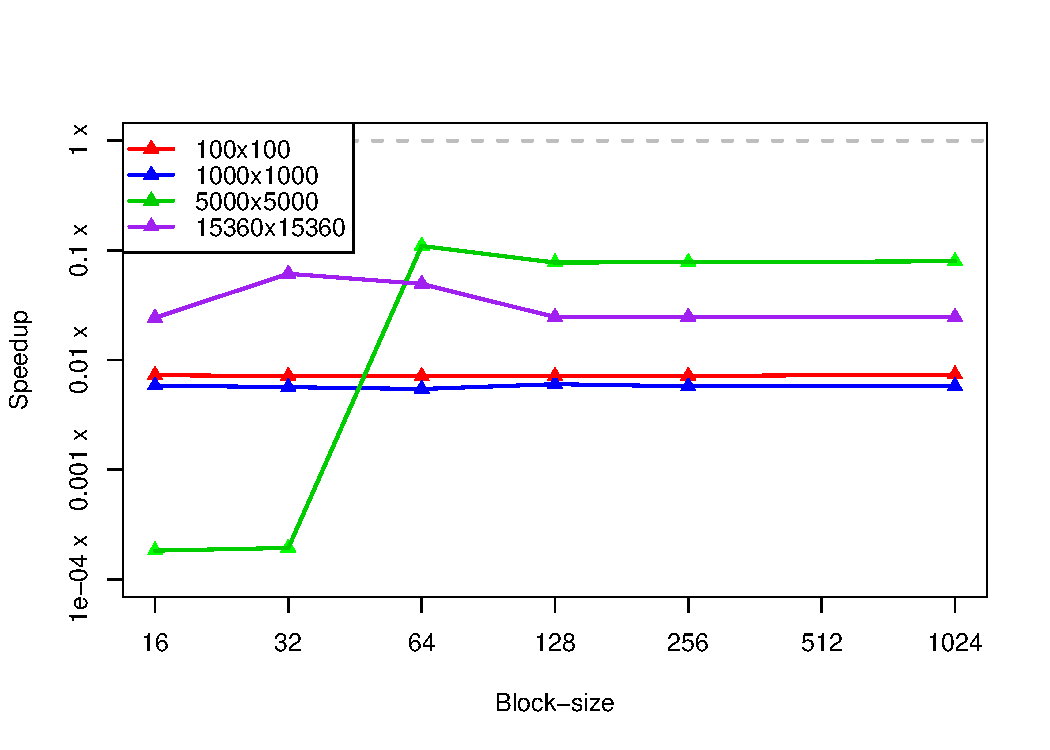
\includegraphics[width=0.85\linewidth]{../plots/alloc_sharedglob.pdf}
		\caption{Speedup of memory allocation time of \texttt{cudaMallocPitch} over \texttt{cudaMalloc}.}
		\label{fig:7}
	\end{subfigure}\hfill
	\begin{subfigure}{0.48\linewidth}
		\centering
		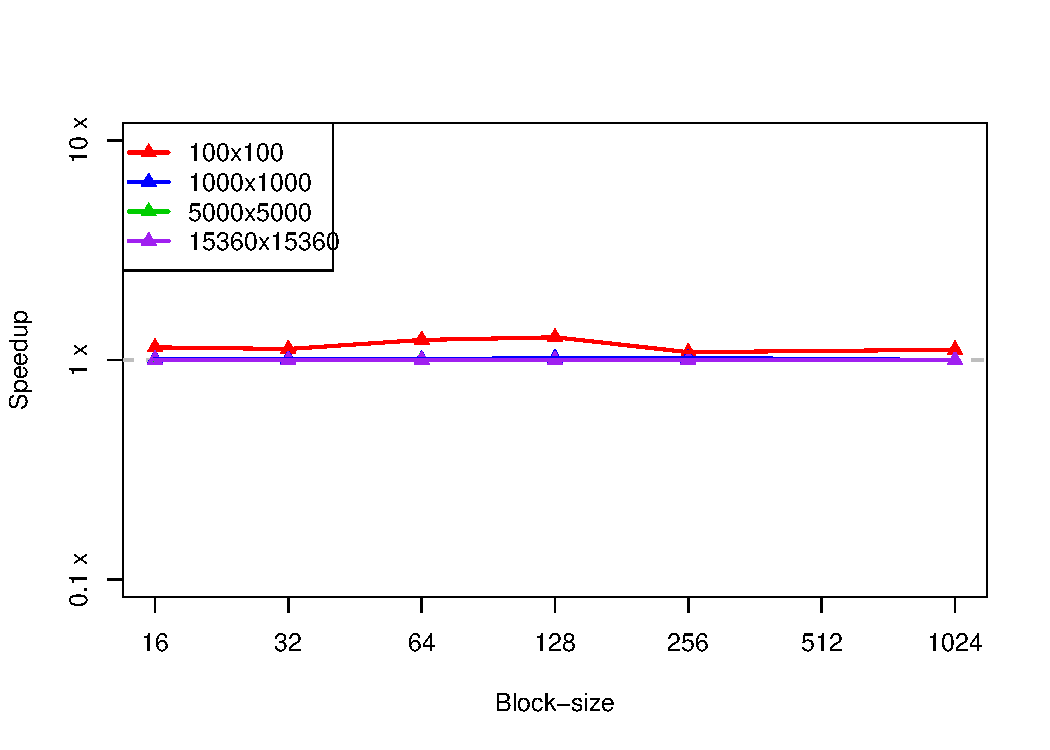
\includegraphics[width=0.85\linewidth]{../plots/RAMsharedglob.pdf}
		\caption{Speedup of device-host transfer time of \texttt{cudaMemcpy2D} over \texttt{cudaMemcpy}.}
		\label{fig:8}
	\end{subfigure}
	\caption{Speedups of allocation time on GPU, and device-host transfer time of \texttt{cudaMallocPitch} and \texttt{cudaMemcpy2D} over \texttt{cudaMalloc} and \texttt{cudaMemcpy}.}
\end{figure}
The allocation time for using \texttt{cudaMalloc} and \texttt{cudaMallocPitch} was tested. Figure \ref{fig:7} would imply that texttt{cudaMalloc} was orders faster, however, in reality it appeared that whatever kernel was ran second in the program actually ran slower. This is contrary to what was seen in the previous assignment where the first kernel was slower and is a result which I cannot come up with justification for.\\
The transfer time from device to host on the other hand was pretty much consistent for both \texttt{cudaMemcpy} and \texttt{cudaMemcpy2D}. No obvious benefits of using 2D data over standard 1D data transfer was seen.
\subsubsection*{SSE}
Both of my CUDA kernels were running succesfully and getting SSEs of $0.00$. However, I changed something in my shared memory kernel and caused a bug which I couldn't find before handing this report in. Due to this, I haven't reported any accuracy values.
\pagebreak
\subsubsection*{Total time}
\begin{figure}
	\centering
	\begin{subfigure}{0.48\linewidth}
		\centering
		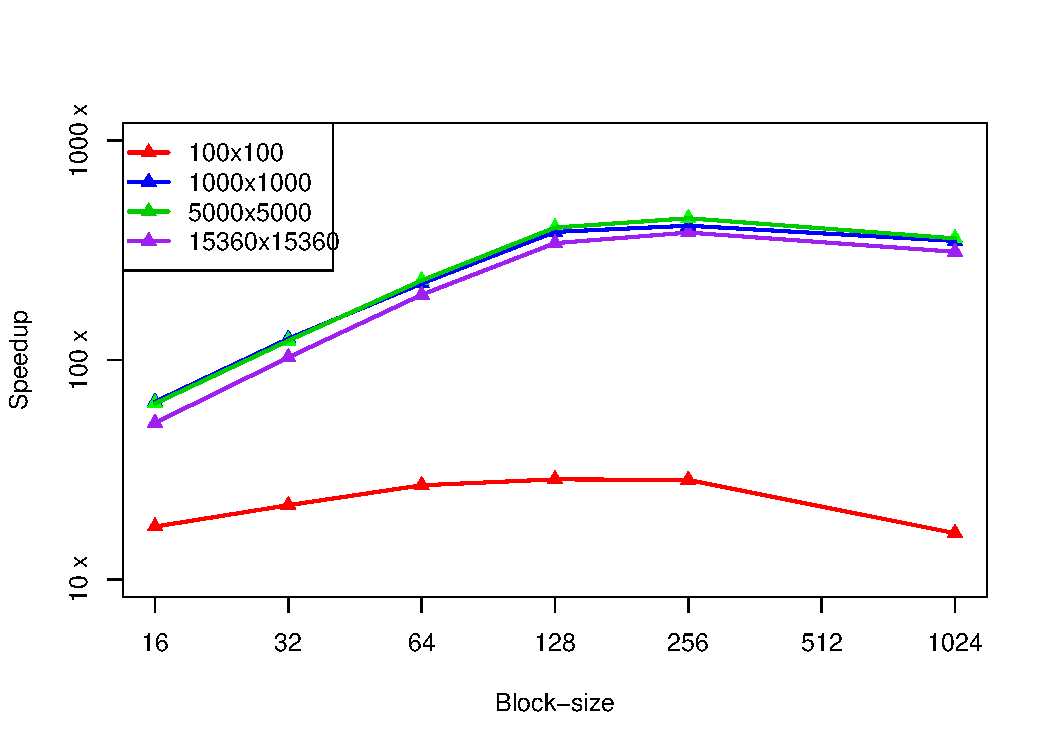
\includegraphics[width=0.85\linewidth]{../plots/tot_shared.pdf}
		\caption{Speedup using shared memory.}
		\label{fig:9}
	\end{subfigure}\hfill
	\begin{subfigure}{0.48\linewidth}
		\centering
		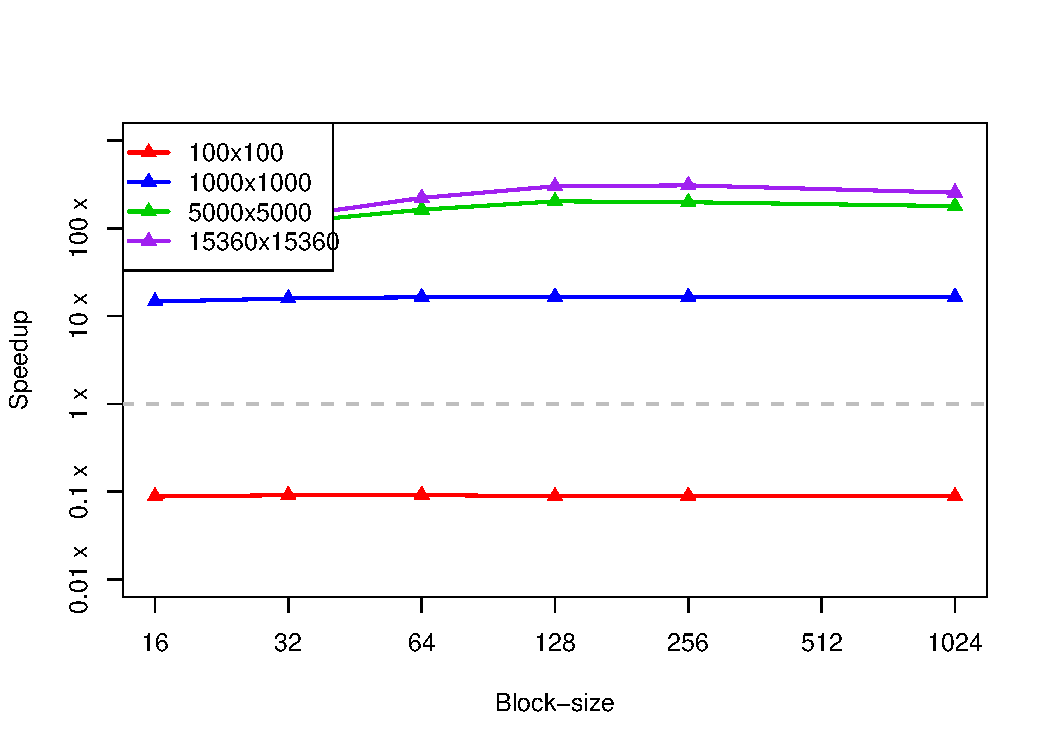
\includegraphics[width=0.85\linewidth]{../plots/tot_glob.pdf}
		\caption{Speedup using global memory.}
		\label{fig:10}
	\end{subfigure}
	\caption{Speedup of total calculation times on GPU, using optimisations and using only global memory.}
\end{figure}
\begin{wrapfigure}{l}{0.5\textwidth}
	\centering
	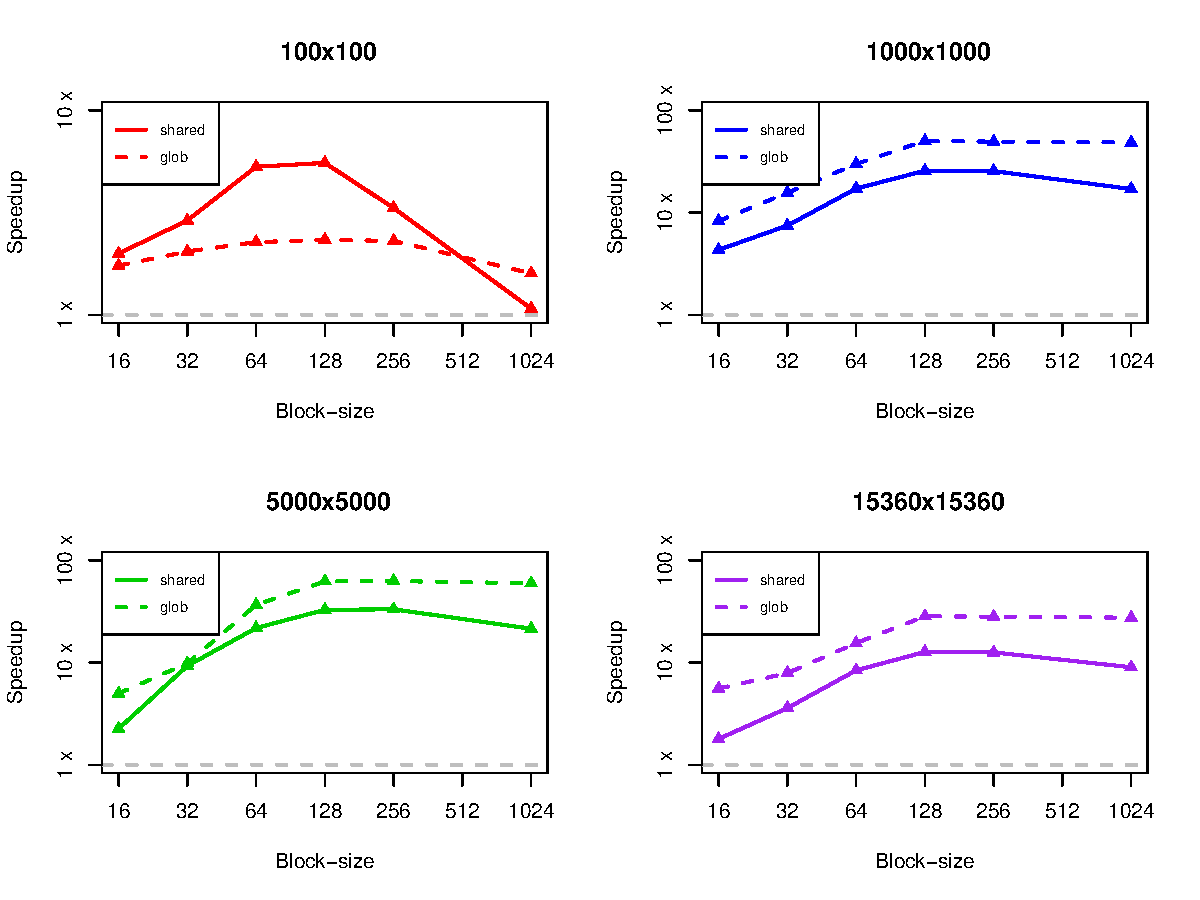
\includegraphics[width=\linewidth]{../plots/tot_globvshared.pdf}
	\caption{Speedup of total calculation time, comparing global memory and optimisations.}
	\label{fig:11}
\end{wrapfigure}
The overall speedups seen are all-in-all, comparable to the results seen in the propagation calculation. The times plateau for global memory and decrease when using shared memory. There is also a reduction for the $15360\times15360$ matrix and global memory proved faster. Overall speedup reached a max of $\sim33\times$ compared to serial. These results are all illustrared in Figures \ref{fig:9}, \ref{fig:10} and \ref{fig:11}.\\
Not entirely sure why using shared memory didn't get more succesful results. Was it possibly due to divergent warps? I struggled to deduce other possible reasons from my code as to why the global memory would be faster.
\subsubsection*{Doubles vs floats}
\begin{figure}
	\centering
	\begin{subfigure}{0.48\linewidth}
		\centering
		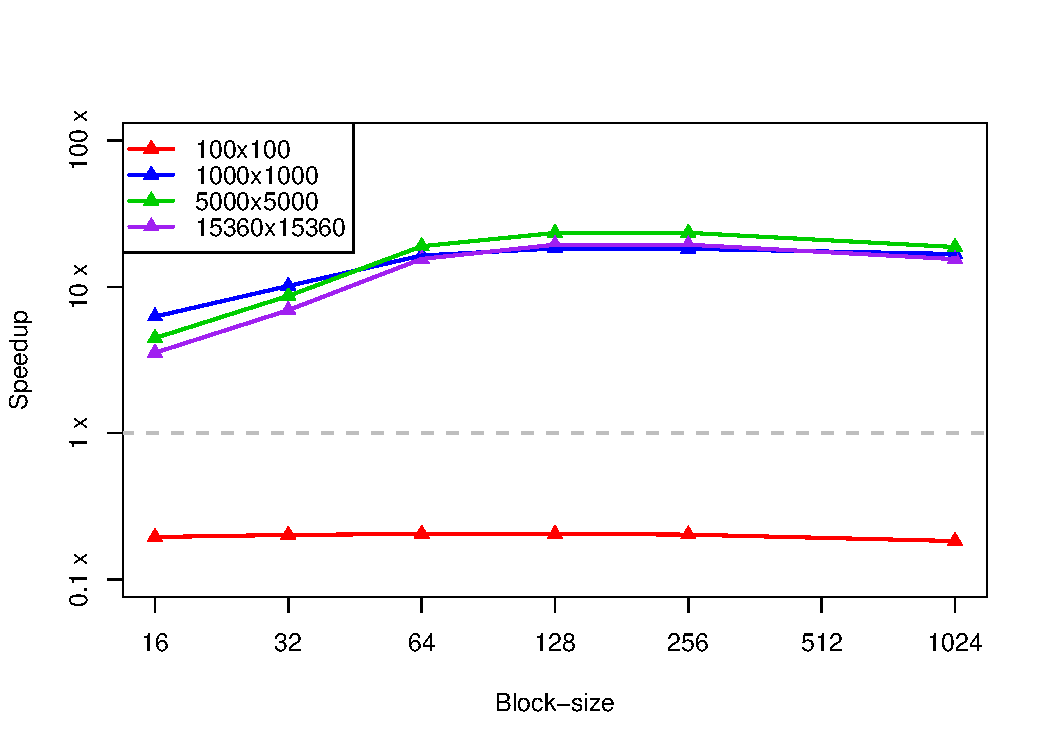
\includegraphics[width=0.85\linewidth]{../plots/tot_double.pdf}
		\caption{Speedup over CPU using double precision numbers.}
		\label{fig:12}
	\end{subfigure}\hfill
	\begin{subfigure}{0.48\linewidth}
		\centering
		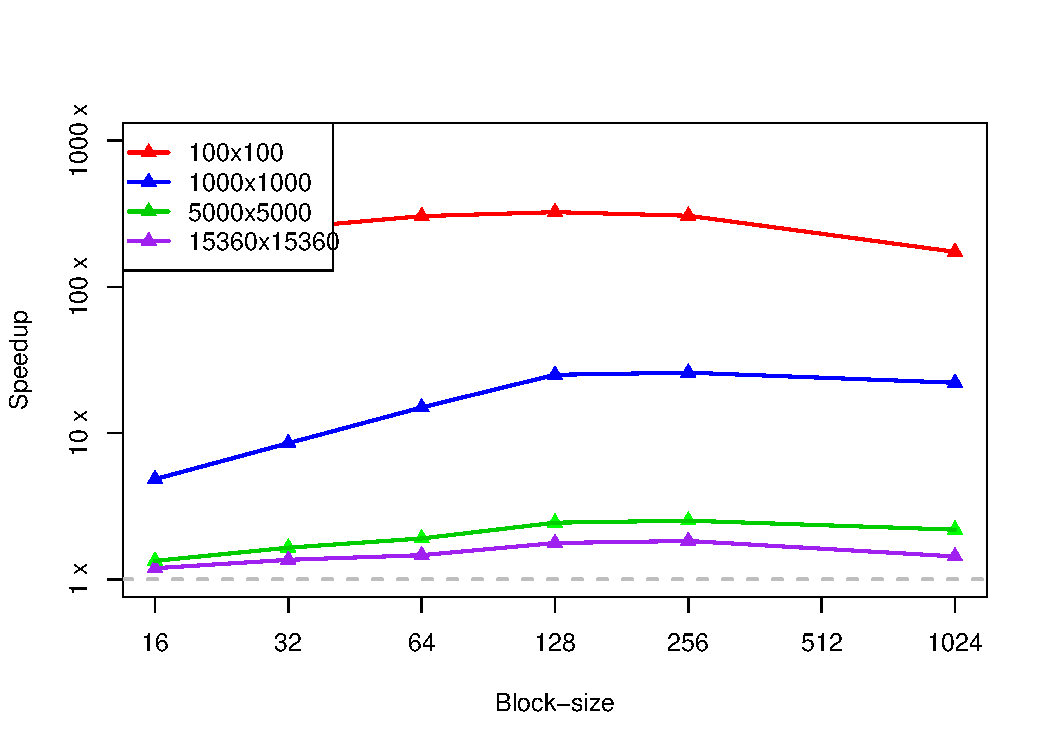
\includegraphics[width=0.85\linewidth]{../plots/tot_doublevfloat.pdf}
		\caption{Speedup of single precision over double precision numbers.}
		\label{fig:13}
	\end{subfigure}
	\caption{Speedup comparisons of floats and doubles.}
\end{figure}
Testing single precision speed versus double precision showed that for 3 or the 4 cases, single precision was slower. Another unexpected result. Shown in Figures \ref{fig:12} and \ref{fig:13}.
\end{document}